\documentclass[11pt,a4paper,twocolumn]{article}
\usepackage[utf8]{inputenc}
\usepackage[english]{babel}
\usepackage[T1]{fontenc}
\usepackage{lmodern}
\usepackage{amsmath}
\usepackage{amsfonts}
\usepackage{amssymb}
\usepackage{graphicx}
\usepackage{booktabs}
\usepackage{array}
\usepackage{geometry}
\usepackage{xcolor}
\usepackage{hyperref}
\usepackage{cite}
\usepackage{listings}
\usepackage{microtype}
\usepackage[font=small,labelfont=bf]{caption}
\usepackage{titlesec}
\usepackage{tikz}
\usetikzlibrary{arrows.meta}

\geometry{top=2.0cm, bottom=2.0cm, left=1.8cm, right=1.8cm}
\graphicspath{{plots/}}

% ---- Visual identity ----
\definecolor{accent}{RGB}{15,82,140}      % deep blue for headings
\definecolor{accentlight}{RGB}{230,238,246}

\hypersetup{colorlinks=true, linkcolor=accent, citecolor=accent, urlcolor=accent}

% Coloured section headings with a rule
\titleformat{\section}{\normalfont\large\bfseries\color{accent}}{\thesection}{0.6em}{}[{\color{accent!30}\titlerule[0.8pt]}]
\titleformat{\subsection}{\normalfont\normalsize\bfseries\color{accent!85!black}}{\thesubsection}{0.5em}{}
\titlespacing*{\section}{0pt}{1.4ex plus 1ex minus .2ex}{1ex}

% Slightly airier rows for readability
\renewcommand{\arraystretch}{1.15}

\title{\textbf{Verification, validation and effective-length estimation of a Helmholtz resonator using an axisymmetric finite-difference solver} \\ \large A GCI convergence study, comparison with published measurements, and a reduced model of the losses}
\author{\textbf{Computational Acoustics Research Project}}
\date{\today}

\begin{document}

\maketitle

\begin{abstract}
This work presents the verification, the validation and the exploitation of a frequency-domain finite-difference (FDM) solver for the Helmholtz equation in axisymmetric cylindrical coordinates $(r,z)$, applied to a Helmholtz resonator; the singularity on the symmetry axis is removed by L'H\^opital's rule. The \emph{code} is verified by a manufactured solution (convergence order $2.03$ on a smooth domain). The \emph{solution} is verified by a Roache GCI study on three grids ($h \in \{2, 1, 0.5\}\text{ mm}$, five neck lengths), completed by a fourth control grid ($0.25$ mm) which confirms the stability both of the observed order ($\approx 0.9$--$1.1$, degraded by the staircase geometry) and of the Richardson extrapolations; the numerical uncertainty is about $2\%$. The \emph{model} is given a first validation against two published experimental configurations (Selamet \emph{et al.}), reproduced to $0.9\%$ and $2.2\%$ with no fitted parameter. The scaling law $f_0(L)$ is then analysed on the extrapolated frequencies, propagating the numerical uncertainty treated as an indicative interval (the GCI not being a statistical standard deviation): an empirical power law and the physical effective-length model, $f_0 = A_H/\sqrt{L + \Delta L_{\mathrm{eff}}}$, are statistically indistinguishable ($\Delta\text{AICc} = 0.3$ to $1.8$ depending on the sample, $5$ to $12$ lengths), yet the physical model is preferred: $A_H = 47.7 \pm 1.4$ is compatible with the theoretical value $48.25$, $\Delta L_{\mathrm{eff}} \approx 0.67$--$0.68\,R_{neck}$ is comparable to the Rayleigh--Ingard correction, and the leave-one-out prediction is ten times better. A baffled-piston radiation-impedance configuration decomposes that correction (interior $0.68\,R_{neck}$; shift $0.823\,R_{neck}$, consistent to $3.1\%$ with the imposed reactance $8R_{neck}/(3\pi)$ --- a consistency test, not an \emph{ab initio} calculation). Finally, a reduced damping model calibrated on the viscothermal boundary-layer estimate ($Q\approx47$) illustrates the signatures of the losses without resolving them.

\vspace{0.5em}
\noindent\textbf{Keywords:} Helmholtz resonator; axisymmetric finite differences; verification and validation; manufactured solution; grid convergence index (GCI); effective length; end correction; viscothermal losses.
\end{abstract}

\vspace{0.4em}
\begingroup
\setcounter{tocdepth}{1}
\renewcommand{\contentsname}{\normalsize\color{accent}\textbf{Contents}}
{\small\tableofcontents}
\endgroup
\vspace{0.4em}
\hrule
\vspace{0.8em}

\section{Introduction and Classical Theory}
The Helmholtz resonator is a fundamental acoustic system \cite{helmholtz1860} consisting of a neck (length $L$, cross-section $S_{neck}$) connected to a rigid cavity of large volume $V_{cav}$. Under an external perturbation the column of air in the neck oscillates as a rigid piston --- an inertial mass effect --- compressing the air in the cavity, which acts as a pneumatic spring.

In the classical one-dimensional, lossless approximation, the natural frequency $f_0$ is given by the free-oscillation formula
\begin{equation}
\label{eq:helmholtz_1d_pure}
f_0 = \frac{c}{2\pi} \sqrt{\frac{S_{neck}}{V_{cav} L}}
\end{equation}
where $c \approx 343\text{ m/s}$ is the speed of sound. For a cylindrical neck of radius $R_{neck}$ and a cylindrical cavity of radius $R_{cav}$ and height $H_{cav}$, the pure theoretical model takes the form of a power law in $L^{-0.5}$:
\begin{equation}
f_0 = \frac{c}{2\pi} \frac{R_{neck}}{R_{cav}} \frac{1}{\sqrt{H_{cav} L}} = \frac{A_H^{\mathrm{th}}}{\sqrt{L}}
\end{equation}
For the reference geometry of this study ($R_{neck}=1\text{ cm}$, $R_{cav}=4\text{ cm}$, $H_{cav}=8\text{ cm}$), the theoretical constant is $A_H^{\mathrm{th}} \approx 48.25\text{ m}^{1/2}/\text{s}$. (The constant of the frequency model is written $A_H$ throughout, the symbol $R_{neck}$ being reserved for the neck radius, so that no notation collides.)

This 1-D theory rests on the assumption of perfect plane waves. It neglects the two-dimensional distortion of the acoustic field at the ends of the neck, which forces the empirical introduction of an end correction $\Delta L$ \cite{rayleigh1896, peters2003end}:
\begin{equation}
\label{eq:helmholtz_correction}
f_0(L) = \frac{c}{2\pi} \sqrt{\frac{S_{neck}}{V_{cav} (L + \Delta L)}} = \frac{A_H^{\mathrm{th}}}{\sqrt{L + \Delta L}}
\end{equation}
where $\Delta L$ is assumed constant for a given neck geometry, of the order of $0.6 \, R_{neck}$ to $0.85 \, R_{neck}$. This work explores how far a physical FDM solver departs from that constant-correction model as the neck length $L$ is varied, and compares its results with reference values from the literature.

\section{Development of the FDM Solver}
\subsection{Frequency-Domain Formulation and Treatment of the Singularity}
Under established harmonic excitation of angular frequency $\omega = 2\pi f$, the complex pressure $p(r,z)$ satisfies the Helmholtz equation in axisymmetric cylindrical coordinates ($\partial p/\partial \theta = 0$):
\begin{equation}
\label{eq:helmholtz_radial}
\frac{\partial^2 p}{\partial r^2} + \frac{1}{r}\frac{\partial p}{\partial r} + \frac{\partial^2 p}{\partial z^2} + k^2 p = 0
\end{equation}
where $k = \omega/c$ is the wavenumber.

The radial term $\frac{1}{r}\frac{\partial p}{\partial r}$ is indeterminate on the axis of revolution $r=0$. Applying L'H\^opital's rule as $r \to 0$,
\begin{equation}
\lim_{r \to 0} \frac{1}{r}\frac{\partial p}{\partial r} = \lim_{r \to 0} \frac{\frac{\partial}{\partial r}\left(\frac{\partial p}{\partial r}\right)}{\frac{\partial}{\partial r}(r)} = \frac{\partial^2 p}{\partial r^2}
\end{equation}
so that on the symmetry axis ($r=0$) the axisymmetric Helmholtz equation simplifies to a regular form:
\begin{equation}
\label{eq:lhopital_axis}
2\frac{\partial^2 p}{\partial r^2} + \frac{\partial^2 p}{\partial z^2} + k^2 p = 0 \quad (\text{with } \frac{\partial p}{\partial r} = 0)
\end{equation}

The boundary conditions applied on the uniform structured grid of the meridian plane $(r,z)$, of spatial step $h$, are:
\begin{itemize}
    \item \textbf{Excitation source} (inlet) at $z=0$, $r \in [0, R_{neck}]$: Dirichlet condition $p(r,0) = p_0 = 1\text{ Pa}$.
    \item \textbf{Symmetry axis} ($r=0$): homogeneous Neumann symmetry condition $\frac{\partial p}{\partial r} = 0$, handled by the regularised stencil \eqref{eq:lhopital_axis}.
    \item \textbf{Rigid walls}: homogeneous Neumann zero-flux condition $\frac{\partial p}{\partial n} = 0$, implemented through virtual solid nodes ($p_{\mathrm{solid}} = p_{\mathrm{fluid}}$).
\end{itemize}

Figure \ref{fig:fdm_grid_nodes} sketches the mesh and the classification of the nodes over the fluid domain of the resonator.

\begin{figure}[ht]
\centering
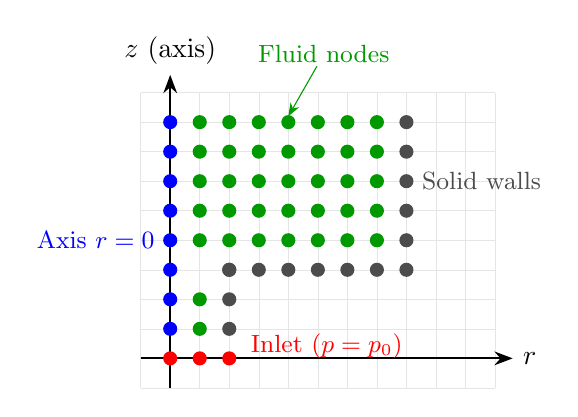
\begin{tikzpicture}[scale=0.75]
    \draw[step=0.5cm, gray!20, very thin] (-0.5,-0.5) grid (5.5,4.5);
    \draw[-{Stealth}, thick] (0,-0.5) -- (0,4.8) node[above] {$z$ (axis)};
    \draw[-{Stealth}, thick] (-0.5,0) -- (5.8,0) node[right] {$r$};

    % Inlet Dirichlet
    \foreach \x in {0, 0.5, 1.0} {
        \node[circle, fill=red, inner sep=1.8pt] at (\x, 0) {};
    }
    \node[red, right] at (1.2,0.2) {\small Inlet ($p=p_0$)};

    % Neumann axis
    \foreach \y in {0.5, 1.0, 1.5, 2.0, 2.5, 3.0, 3.5, 4.0} {
        \node[circle, fill=blue, inner sep=1.8pt] at (0, \y) {};
    }
    \node[blue, left] at (-0.1, 2.0) {\small Axis $r=0$};

    % Solid boundary
    \foreach \y in {0.5, 1.0, 1.5} {
        \node[circle, fill=black!70, inner sep=1.8pt] at (1.0, \y) {};
    }
    \foreach \x in {1.0, 1.5, 2.0, 2.5, 3.0, 3.5, 4.0} {
        \node[circle, fill=black!70, inner sep=1.8pt] at (\x, 1.5) {};
    }
    \foreach \y in {2.0, 2.5, 3.0, 3.5, 4.0} {
        \node[circle, fill=black!70, inner sep=1.8pt] at (4.0, \y) {};
    }
    \node[black!70, right] at (4.1, 3.0) {\small Solid walls};

    % Fluid nodes
    \foreach \x in {0.5} {
        \foreach \y in {0.5, 1.0} {
            \node[circle, fill=green!60!black, inner sep=1.8pt] at (\x, \y) {};
        }
    }
    \foreach \x in {0.5, 1.0, 1.5, 2.0, 2.5, 3.0, 3.5} {
        \foreach \y in {2.0, 2.5, 3.0, 3.5, 4.0} {
            \node[circle, fill=green!60!black, inner sep=1.8pt] at (\x, \y) {};
        }
    }
    \node[green!60!black, fill=white, inner sep=1pt] (lblfluid) at (2.6, 5.15) {\small Fluid nodes};
    \draw[green!60!black, -{Stealth}, thin] (lblfluid) -- (2.0, 4.1);
\end{tikzpicture}
\caption{Geometric classification of the nodes and boundary conditions on the axisymmetric FDM domain.}
\label{fig:fdm_grid_nodes}
\end{figure}

\section{Mesh Convergence Study}
\label{sec:convergence}
To quantify the spatial discretisation error, the natural frequency $f_0$ is solved on three grids of decreasing spatial step at a constant ratio ($h \in \{2, 1, 0.5\}\text{ mm}$, refinement ratio $r = 2$) for the five neck lengths of the study, $L \in \{2, 3, 4, 5, 6\}\text{ cm}$. The results are collected in Table \ref{tab:mesh_sensitivity}.

\begin{table*}[t]
\centering
\caption{Natural frequencies $f_0$ (Hz) of the FDM solver on the three refinement grids}
\label{tab:mesh_sensitivity}
\begin{tabular}{c*{6}{>{\centering\arraybackslash}p{1.8cm}}}
\toprule
L (cm) & \multicolumn{2}{c}{$h = 2\text{ mm}$} & \multicolumn{2}{c}{$h = 1\text{ mm}$} & \multicolumn{2}{c}{$h = 0.5\text{ mm}$} \\
\cmidrule(r){2-3} \cmidrule(lr){4-5} \cmidrule(l){6-7}
 & $f_0$ (Hz) & Nodes & $f_0$ (Hz) & Nodes & $f_0$ (Hz) & Nodes \\
\midrule
2.0 & 309.9 & 1\,071 & 301.4 & 4\,141 & 297.0 & 16\,281 \\
3.0 & 264.6 & 1\,176 & 257.4 & 4\,551 & 253.6 & 17\,901 \\
4.0 & 234.6 & 1\,281 & 228.2 & 4\,961 & 224.8 & 19\,521 \\
5.0 & 212.9 & 1\,386 & 207.0 & 5\,371 & 203.9 & 21\,141 \\
6.0 & 196.1 & 1\,491 & 190.7 & 5\,781 & 187.9 & 22\,761 \\
\bottomrule
\end{tabular}
\end{table*}

A systematic decrease of the natural frequency is observed as the grid is refined, consistent with a better representation of the neck--cavity transition and of the effective acoustic mass. To quantify the discretisation error objectively, Roache's methodology based on the Grid Convergence Index (GCI) is applied \cite{roache1994perspective}. From the frequencies on the three grids ($f_1$ fine, $f_2$ intermediate, $f_3$ coarse), the observed order of convergence $p$, the Richardson extrapolation $f_{h\to0}$ and the GCI numerical uncertainty of the fine grid are
\begin{align}
p &= \frac{\ln\left(|f_3 - f_2|/|f_2 - f_1|\right)}{\ln r}, \quad
f_{h\to0} = f_1 + \frac{f_1 - f_2}{r^p - 1} \\
\mathrm{GCI}_{\mathrm{fine}} &= F_s\,\frac{|(f_2 - f_1)/f_1|}{r^p - 1}, \quad F_s = 1.25
\end{align}
The results are listed in Table \ref{tab:gci}.

\begin{table}[h]
\centering
\caption{Mesh convergence: observed order $p$, Richardson extrapolation and GCI uncertainty on the fine grid}
\label{tab:gci}
\begin{tabular}{ccccc}
\toprule
$L$ (cm) & $f_{0,\,\mathrm{fine}}$ (Hz) & $p$ & $f_{h\to0}$ (Hz) & GCI (\%) \\
\midrule
2.0 & 297.0 & 0.913 & 291.9 & 2.14 \\
3.0 & 253.6 & 0.949 & 249.6 & 1.99 \\
4.0 & 224.8 & 0.867 & 220.6 & 2.34 \\
5.0 & 203.9 & 0.943 & 200.6 & 2.04 \\
6.0 & 187.9 & 0.933 & 184.7 & 2.07 \\
\bottomrule
\end{tabular}
\end{table}

The observed order of convergence, $p \approx 0.92$, is close to $1$: although the interior stencil is formally second order, the staircase representation of the walls and of the neck--cavity junction degrades the convergence towards first order. The numerical uncertainty on the finest grid is of the order of $2\%$. The Richardson extrapolation provides the reference estimate used in what follows; its reliability nevertheless presupposes a near-asymptotic regime, an assumption checked as follows.

\paragraph{Check of the asymptotic regime (fourth grid).} An additional grid at $h=0.25$ mm is computed for $L=2$ and $4$ cm (up to $77\,441$ nodes), giving two refinement triplets per length. The observed order remains stable ($p = 0.913 \to 0.996$ for $L=2$ cm; $0.867 \to 1.013$ for $L=4$ cm) and the Richardson extrapolations of the two triplets agree to $0.20\%$ and $0.36\%$ respectively --- far below the GCI --- while the GCI of the finest grid falls to about $1\%$. The extrapolated references used below are therefore stable at the level of precision required, without strict asymptotic independence being claimed.

This \emph{solution verification} (order $\approx 1$, limited by the geometry) must be distinguished from \emph{code verification} \cite{roache1998verification}. The latter is established by a manufactured solution (MMS): on a smooth rectangular domain with no staircase, an analytic solution regular on the axis is imposed through a source term, and the $L_2$ error decreases at \textbf{order $2.03$} over four grids ($h \in \{4, 2, 1, 0.5\}$ mm), confirming that the axisymmetric stencil really is second order. The loss of one order on the real resonator is therefore attributable mainly to the staircase discretisation of the geometry --- without excluding secondary contributions from the treatment of corners and Neumann conditions, or from peak extraction --- and not to a programming error.

\section{A First Validation Against Two Published Experimental Configurations}
\label{sec:validation}
Verification --- of the code by MMS, of the solution by GCI --- says nothing about whether the model matches physical reality: that is the role of \emph{validation}. In the absence of a dedicated experimental campaign, the solver is compared with the published measurements of Selamet \emph{et al.} \cite{selamet1997circular}, whose configuration --- a cylindrical neck opening into a coaxial cylindrical cavity --- is exactly that of the present axisymmetric model: neck $d_c = 4.044$ cm, $l_c = 8.5$ cm, fixed volume $V = 4500\text{ cm}^3$, variable cavity length-to-diameter ratio $l/d$. The resonance frequencies there are measured in an impedance tube (transmission-loss peak) and confirmed by a 3-D boundary-element method to within barely 1 Hz.

At the resonance of a side branch the input impedance of the neck vanishes ($p\approx0$ at the mouth), so the Dirichlet condition of the solver is the adequate representation of this configuration, all the more as the neck occupies $83\%$ of the tube diameter, making the tube-side end correction marginal. Table \ref{tab:selamet} compares the computed natural frequencies, with no fitted parameter, against the published values.

\begin{table}[h]
\centering
\caption{Validation against Selamet \emph{et al.} \cite{selamet1997circular} ($V=4500$ cm$^3$, grid $h=1$ mm)}
\label{tab:selamet}
\begin{tabular}{lcccc}
\toprule
Config. & Cavity $d_v \times l_v$ (cm) & published $f_r$ (Hz) & FDM (Hz) & Deviation \\
\midrule
$l/d=1.0$ & $17.9 \times 17.9$ & $91$ & $93.0$ & $2.2\%$ \\
$l/d=10$ & $8.3 \times 83.1$ & $72$ & $72.7$ & $0.9\%$ \\
\bottomrule
\end{tabular}
\end{table}

The deviations ($0.9\%$ and $2.2\%$) are of the same order as the GCI numerical uncertainty ($\approx2\%$), the rounding of the published values ($\pm0.5$ Hz) and the neglected neck--tube interface correction. This remains a \emph{first} validation, and its scope should be stated precisely: it rests on two configurations only, it concerns the resonance frequency alone rather than the full shape of the response, and the experimental uncertainties of the published measurements and dimensions are not available. The solver nevertheless reproduces independent measurements, with no fitted parameter, on a geometry about four times larger than that of the main study; a broader validation --- several neck-to-cavity ratios, the complete frequency response, and a dedicated experimental campaign following the protocol supplied with the repository --- remains necessary.

\section{Frequency Responses and Extraction of \texorpdfstring{$f_0$}{f0}}
To identify the natural frequency $f_0$, the excitation frequency $f$ is swept and the maximum of the normalised mean cavity pressure is sought. That pressure is volume-averaged over the cavity domain ($V_{cav}$) in the axisymmetric formulation:
\begin{equation}
p_{avg}(f) = \frac{\iint_{V_{cav}} p(r,z,f) 2\pi r \, dr \, dz}{\iint_{V_{cav}} 2\pi r \, dr \, dz} \approx \frac{\sum_{i} p_i r_i}{\sum_{i} r_i}
\end{equation}
where the index $i$ runs over every fluid node of the cavity.

\begin{figure}[ht]
\centering
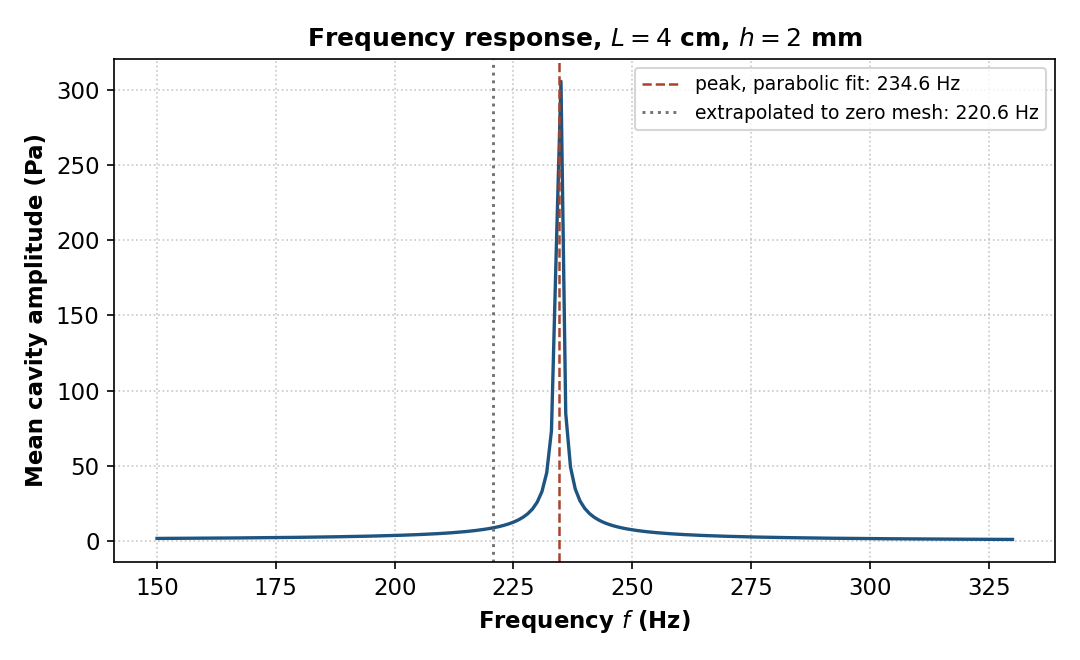
\includegraphics[width=0.48\textwidth]{doe_resonance.png}
\caption{Frequency response of the mean cavity amplitude for the reference geometry $L=4$ cm, \emph{on the coarse grid} $h=2$ mm: the peak ($234.6$ Hz by parabolic interpolation, identical to Table \ref{tab:mesh_sensitivity}) gives $f_0$ for that grid; the value extrapolated to zero mesh size is $220.6$ Hz (Table \ref{tab:gci}).}
\label{fig:freq_response}
\end{figure}

Figure \ref{fig:freq_response} shows the amplitude response for $L=4\text{ cm}$, obtained by a frequency sweep of the solver on the $h=2$ mm grid. The resonance peak $f_0$ is extracted by parabolic interpolation around the maximum. One point matters for the consistency of this article: each grid has its own peak frequency (Table \ref{tab:mesh_sensitivity}), so wherever a value of $f_0$ is used below, the corresponding grid is stated.

\section{Identification of the Scaling Law}
Table \ref{tab:f0_comparison} gathers the natural resonance frequencies $f_0(L)$ obtained for five neck lengths.

\begin{table*}[t]
\centering
\caption{Comparison of the natural resonance frequencies $f_0$ (Hz) for five neck lengths}
\label{tab:f0_comparison}
\begin{tabular}{c*{3}{>{\centering\arraybackslash}p{3cm}}}
\toprule
L (cm) & 1-D theory ($\Delta L=0$) & Fine FDM ($h=0.5$ mm) & Extrapolated FDM ($h\to0$)\\
\midrule
2.0 & 341.2 & 297.0 & 291.9 \\
3.0 & 278.6 & 253.6 & 249.6 \\
4.0 & 241.3 & 224.8 & 220.6 \\
5.0 & 215.8 & 203.9 & 200.6 \\
6.0 & 197.0 & 187.9 & 184.7 \\
\bottomrule
\end{tabular}
\end{table*}

To identify the geometric scaling law, two two-parameter models are compared \emph{on equal terms}: an empirical power law (A) and the physical Helmholtz model with an \emph{effective length} (B),
\begin{equation}
\underbrace{f_0(L) = A\, L^b}_{\text{(A) power law}}
\qquad
\underbrace{f_0(L) = \frac{A_H}{\sqrt{L + \Delta L_{\mathrm{eff}}}}}_{\text{(B) effective length}}
\end{equation}
A methodological point: the FDM frequencies carry a numerical uncertainty of about $2\%$ (Section \ref{sec:convergence}), far larger than the residuals of the fit. The fit is therefore performed on the \emph{Richardson-extrapolated} frequencies (Table \ref{tab:f0_comparison}), \emph{weighted} by the GCI uncertainties. The status of that weighting needs to be stated: the GCI is a \emph{conservative bound} on the discretisation error, not a random Gaussian standard deviation, and the errors at different lengths are most likely \emph{correlated} (same code, same meshes, same extrapolation). It is nevertheless treated as an indicative independent $\sigma$ --- an explicitly approximate assumption --- so that the reduced $\chi^2$, the AICc and the parameter intervals should be read as a \emph{sensitivity analysis over numerical intervals} rather than as strict probabilistic inference; the $\chi^2/\mathrm{dof}$ values well below 1 are themselves a reflection of how conservative the GCI is. Leave-one-out (LOO) cross-validation, which does not depend on that error model, completes the comparison. The results appear in Table \ref{tab:model_selection}.

\begin{table*}[t]
\centering
\caption{Fit weighted by the numerical uncertainty ($k=2$ parameters; reduced $\chi^2$, AICc and leave-one-out prediction error)}
\label{tab:model_selection}
\begin{tabular}{>{\raggedright\arraybackslash}p{4.5cm}>{\centering\arraybackslash}p{5cm}>{\centering\arraybackslash}p{1.8cm}>{\centering\arraybackslash}p{1.6cm}>{\centering\arraybackslash}p{2.4cm}}
\toprule
Model & Fitted parameters & $\chi^2/\mathrm{dof}$ & AICc & LOO-RMSE (Hz) \\
\midrule
(A) Power law $A L^b$ & $A=57.4\pm4.6$, \; $b=-0.417\pm0.024$ & $0.09$ & $10.3$ & $2.97$ \\
(B) Effective length $A_H/\sqrt{L+\Delta L_{\mathrm{eff}}}$ & $A_H=47.7\pm1.4$, \; $\Delta L_{\mathrm{eff}}=6.7\pm2.4$ mm & $<0.01$ & $10.0$ & $\mathbf{0.58}$ \\
\bottomrule
\end{tabular}
\end{table*}

Once the numerical uncertainty is propagated, both models are \emph{compatible} with the data ($\chi^2/\mathrm{dof} < 1$) and the gap $\Delta\text{AICc} = \text{AICc}_A - \text{AICc}_B \approx 0.3$ is \emph{not decisive}: at this level of uncertainty the data alone cannot statistically separate the two forms. The physical model (B) is nevertheless preferred, for three converging reasons:
\begin{itemize}
    \item its fitted constant $A_H = 47.7 \pm 1.4$ is compatible with the \emph{a priori} theoretical constant $A_H^{\mathrm{th}} = 48.25$;
    \item its effective length $\Delta L_{\mathrm{eff}} = 6.7\text{ mm} \approx 0.67\,R_{neck}$ is of the same order as the Rayleigh--Ingard end correction \cite{ingard1953theory} ($0.6$--$0.85\,R_{neck}$) --- \emph{indicatively}, the model containing no exterior radiation domain (see below);
    \item its out-of-sample predictive capacity is markedly better (LOO-RMSE $0.6$ against $3.0$ Hz).
\end{itemize}

The apparent exponent $b \approx -0.42$ of a power law is therefore not an alternative physics: a function in $1/\sqrt{L+\Delta L_{\mathrm{eff}}}$, observed over a restricted range of $L$, is locally indistinguishable from a power law of intermediate exponent. Finally, $\Delta L_{\mathrm{eff}}$ is an \emph{effective} correction specific to the numerical configuration: it aggregates the neck--cavity transition, the Dirichlet inlet condition and the staircase discretisation, and does not constitute a verification of the radiation end correction in the strict sense.

To go beyond the limitation of a small sample, the analysis is repeated on an enlarged set of twelve neck lengths ($1.5$ to $7.0$ cm). The trend strengthens: $\Delta\text{AICc}$ rises from $0.3$ to $\approx 1.8$ in favour of the effective-length model, whose parameters remain stable ($A_H = 48.6 \approx A_H^{\mathrm{th}}$, $\Delta L_{\mathrm{eff}} = 0.68\,R_{neck}$) and whose out-of-sample prediction is far better (LOO-RMSE $0.3$ against $3.3$ Hz). The gap nevertheless stays below the threshold of strong exclusion ($\Delta\text{AICc}>10$): the physical model is \emph{favoured} without being formally the only admissible one.

\subsection{Interior/Exterior Decomposition by a Radiation-Impedance Condition}
\label{sec:radiation}
To separate the interior part of $\Delta L_{\mathrm{eff}}$ from the exterior radiation load, a second configuration is built: the mouth ($z=0$, $r\leq R_{neck}$) is no longer a Dirichlet boundary but carries the low-frequency radiation impedance of a baffled piston \cite{rayleigh1896, morse1968theoretical},
\begin{equation}
Z_{\mathrm{rad}} = \rho c\left[\tfrac{1}{2}(kR_{neck})^2 + i\,\tfrac{8}{3\pi}\,kR_{neck}\right],
\end{equation}
imposed through a Robin condition ($\partial p/\partial z = i\omega\rho\, p/Z_{\mathrm{rad}}$, ghost node), the excitation becoming a volume forcing inside the cavity. The imaginary part of $Z_{\mathrm{rad}}$ analytically encodes the exterior correction $\Delta L_{\mathrm{ext}} = 8R_{neck}/(3\pi) \approx 0.849\,R_{neck}$; its real part introduces radiation damping.

Both configurations are solved on the \emph{same} grid ($h=1$ mm) for five lengths, so that the discretisation bias cancels to first order in the difference. The fit gives $\Delta L_{\mathrm{Dirichlet}} = 0.676\,R_{neck}$ and $\Delta L_{\mathrm{radiation}} = 1.499\,R_{neck}$, a shift of $0.823\,R_{neck}$, agreeing to $3.1\%$ with the analytic value $8/(3\pi) = 0.849$. This result is \emph{consistent} with the additive decomposition $\Delta L_{\mathrm{tot}} = \Delta L_{\mathrm{int}} + \Delta L_{\mathrm{ext}}$, and identifies at the same time $\Delta L_{\mathrm{int}} \approx 0.68\,R_{neck}$ as the correction proper to the neck--cavity junction. Its scope should be stated honestly: since the imposed reactance \emph{contains} $8R_{neck}/(3\pi)$, this test essentially shows that the Robin condition is correctly implemented and that the chain of computation, extraction and regression recovers the imposed variation. It is a consistency check, not an \emph{ab initio} calculation of radiation, which would require a meshed exterior domain with a Sommerfeld condition or a perfectly matched layer (PML) \cite{berenger1994perfectly}. That calculation is carried out in the companion transient study of the repository. The radiation quality factor measured on these responses ($Q_{\mathrm{rad}} \approx 150$--$320$, increasing as $f_0$ decreases) further confirms that radiation is a secondary loss channel compared with the viscothermal losses ($Q_{\mathrm{visc}}\approx47$, Section \ref{sec:losses}).

\begin{figure*}[ht]
\centering
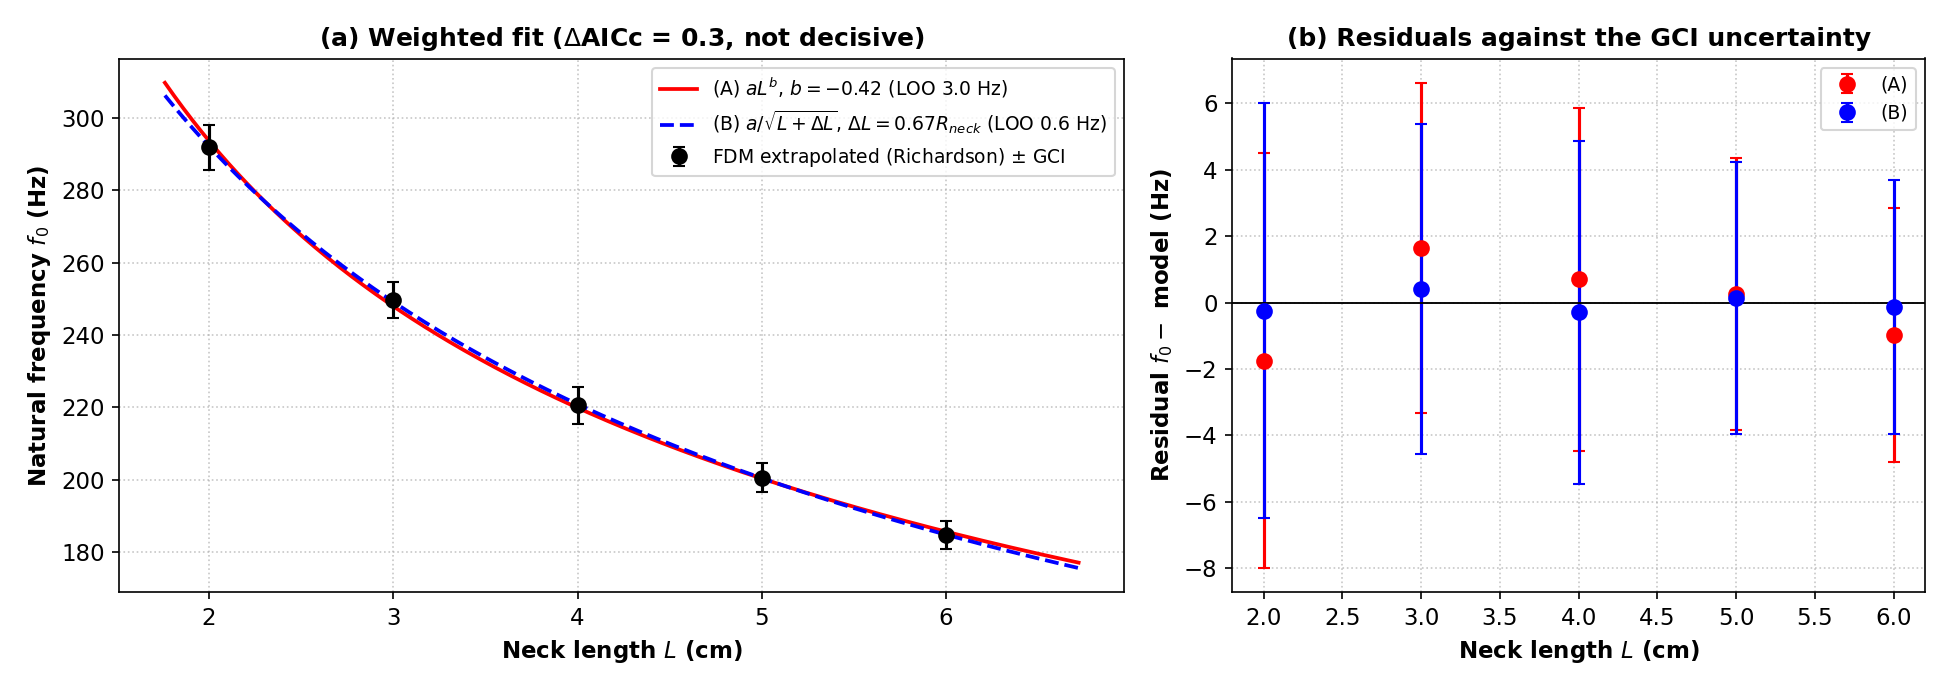
\includegraphics[width=0.95\textwidth]{scaling_law_gci.png}
\caption{(a) Fit weighted by the numerical uncertainty: Richardson-extrapolated frequencies with GCI uncertainty bars ($\approx 2\%$), the effective-length model (blue) and the power law (red). Both models stay within the error bars ($\Delta$AICc not decisive); the effective length nevertheless predicts markedly better out of sample (LOO). (b) Residuals of the two models relative to the GCI uncertainty.}
\label{fig:scaling_gci}
\end{figure*}

Figure \ref{fig:scaling_gci}(a) illustrates these fits. The main scientific limitations of this study remain the small number of geometries tested (five lengths), the residual numerical uncertainty ($\approx 2\%$, see Section \ref{sec:convergence}), the staircase geometry at the neck--cavity junction, and the absence of a direct experimental comparison.

\section{Viscothermal Losses and Quality Factor}
\label{sec:losses}
The frequency-domain solver above is lossless: its resonance is undamped, and the apparent width in Figure \ref{fig:freq_response} is due only to the finite resolution of the sweep. To introduce damping, the \emph{damped} wave equation is solved in the transient regime by an explicit leapfrog scheme,
\begin{equation}
\frac{\partial^2 p}{\partial t^2} + \gamma(r,z)\frac{\partial p}{\partial t} = c^2\!\left(\frac{\partial^2 p}{\partial r^2} + \frac{1}{r}\frac{\partial p}{\partial r} + \frac{\partial^2 p}{\partial z^2}\right),
\end{equation}
comparing two dissipation mechanisms.

\subsection{Bulk (Stokes) Losses: Negligible}
Classical absorption in air --- shear and bulk viscosity, thermal conduction --- gives the Stokes attenuation coefficient $\alpha = \delta_{\mathrm{diff}}\,\omega^2/(2c^3)$ \cite{stokes1845theories}, that is a uniform damping $\gamma_{\mathrm{bulk}} = \delta_{\mathrm{diff}}\,\omega^2/c^2$. With a sound diffusivity $\delta_{\mathrm{diff}}\approx 3.8\times10^{-5}\text{ m}^2/\text{s}$, the associated quality factor reaches $Q_{\mathrm{bulk}}\approx 2\times10^{6}$: at centimetre scales this mechanism is entirely negligible.

\subsection{Viscothermal Boundary-Layer Losses: Dominant}
The real mechanism is viscous friction and thermal conduction in the thin acoustic boundary layer on the walls of the \emph{neck}, where the particle velocity is largest \cite{crandall1926theory, morse1968theoretical}. An energy balance --- the energy of the mode against the power dissipated on the neck wall, of surface resistance $R_s=\sqrt{\rho\mu\omega/2}\,[1+(\gamma-1)/\sqrt{Pr}]$ --- leads to the analytic quality factor
\begin{equation}
\label{eq:Qvisc}
Q_{\mathrm{visc}} = \frac{R_{neck}}{F_t\,\delta_v}, \quad \delta_v=\sqrt{\frac{2\mu}{\rho\,\omega_0}}, \quad F_t = 1+\frac{\gamma-1}{\sqrt{Pr}}\approx 1.48,
\end{equation}
where $\delta_v$ is the viscous boundary-layer thickness. The transient study is run on the $h=2$ mm grid, whose natural frequency is $f_0 = 234.6\text{ Hz}$ (Table \ref{tab:mesh_sensitivity}): it is that value --- not the extrapolated $221.0$ Hz --- which sets the excitation and $\delta_v\approx0.14\text{ mm}$, whence $Q_{\mathrm{visc}}\approx47$. The $6\%$ gap between the two frequencies would change $Q_{\mathrm{visc}}$ by only about $3\%$ ($Q\propto\sqrt{f_0}$), with no bearing on the conclusions. The value obtained is consistent with measurements on real resonators (next section).

The transient solver does not implement this sub-millimetre boundary layer, which would require $h<0.1\text{ mm}$. It uses a \emph{reduced equivalent-damping model}: a term $\gamma$ localised in the neck, whose amplitude is \emph{calibrated} so that the quality factor of the free decay reproduces $Q_{\mathrm{visc}}$. Re-measuring the stored ring-down with a logarithmic decrement on the Hilbert envelope --- the same estimator the experimental protocol of the repository applies to a real recording --- returns $Q = 45.8$ against the calibration target of $47.4$. The two estimators of one and the same decay differ by $3.4\%$, which is a fair statement of how precisely a $Q$ can be read off a trace only three time constants long. Either way the number is not an independent validation but a \emph{consistency check} of the calibration. For the same reason the dissipation map that appeared in an earlier version of Figure \ref{fig:losses} has been dropped: it reproduced the \emph{imposed} localisation of $\gamma$ rather than any spontaneous emergence, and so illustrated an input rather than a result. What remains of the reduced model is what it can legitimately show: that only the neck mechanism damps at all, at what rate, and how little of that rate a finite observation window lets a spectrum resolve (Figure \ref{fig:losses}).

\begin{figure*}[t]
\centering
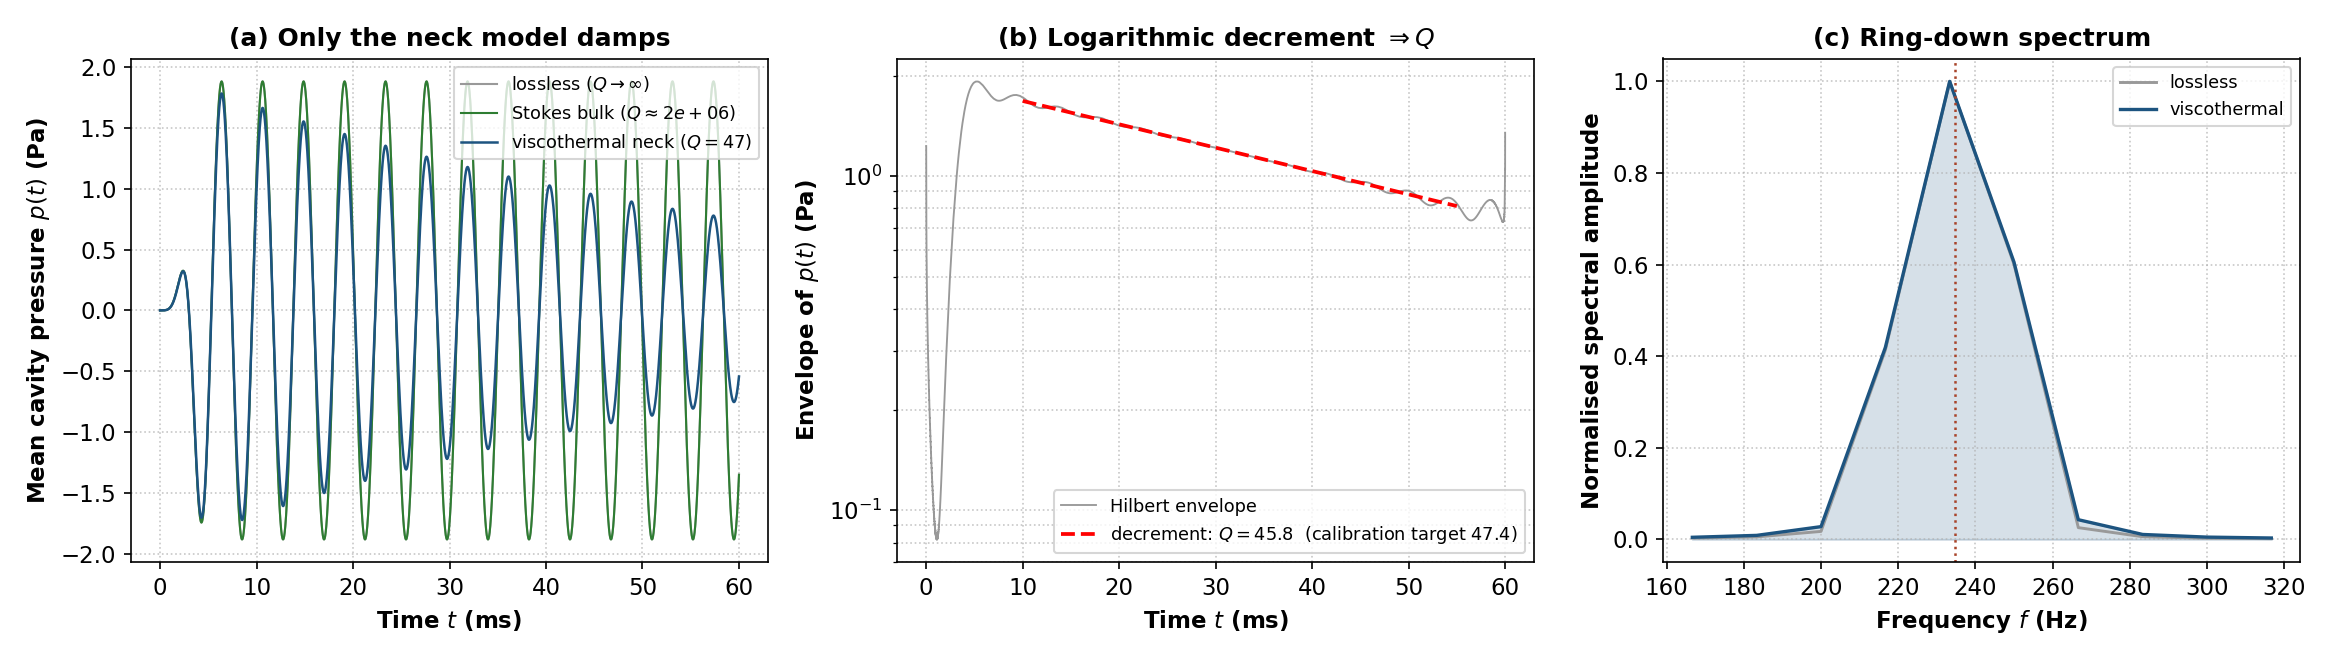
\includegraphics[width=0.92\textwidth]{phase1_losses.png}
\caption{Losses of the resonator ($L=4$ cm), with a calibrated reduced equivalent-damping model. (a) Impulse response: only the viscothermal neck model damps, the bulk model being indistinguishable from the lossless case. (b) Hilbert envelope on a logarithmic scale and its least-squares slope, giving $Q=45.8$ against the calibration target $47.4$. (c) Ring-down spectrum: its visible width is dominated by the finite observation window ($\approx 4/T$) and does not resolve the physical broadening $\Delta f=f_0/Q\approx5$ Hz, which is why $Q$ is measured in the time domain (panel b).}
\label{fig:losses}
\end{figure*}

\subsection{Comparison with the Literature}
For all five geometries, the FDM natural frequency falls inside Ingard's end-correction band $\Delta L\in[0.60;0.85]\,R_{neck}$ \cite{ingard1953theory} (Figure \ref{fig:verif}a). The quality factor $Q\approx47$ is compatible with values measured on real resonators ($Q\sim30$--$70$, Moloney \cite{moloney2004quality}), and the scaling law $Q_{\mathrm{visc}}\propto\sqrt{\omega_0}$ reproduces the expected trend: higher-pitched resonators are less damped (Figure \ref{fig:verif}b).

\begin{figure*}[t]
\centering
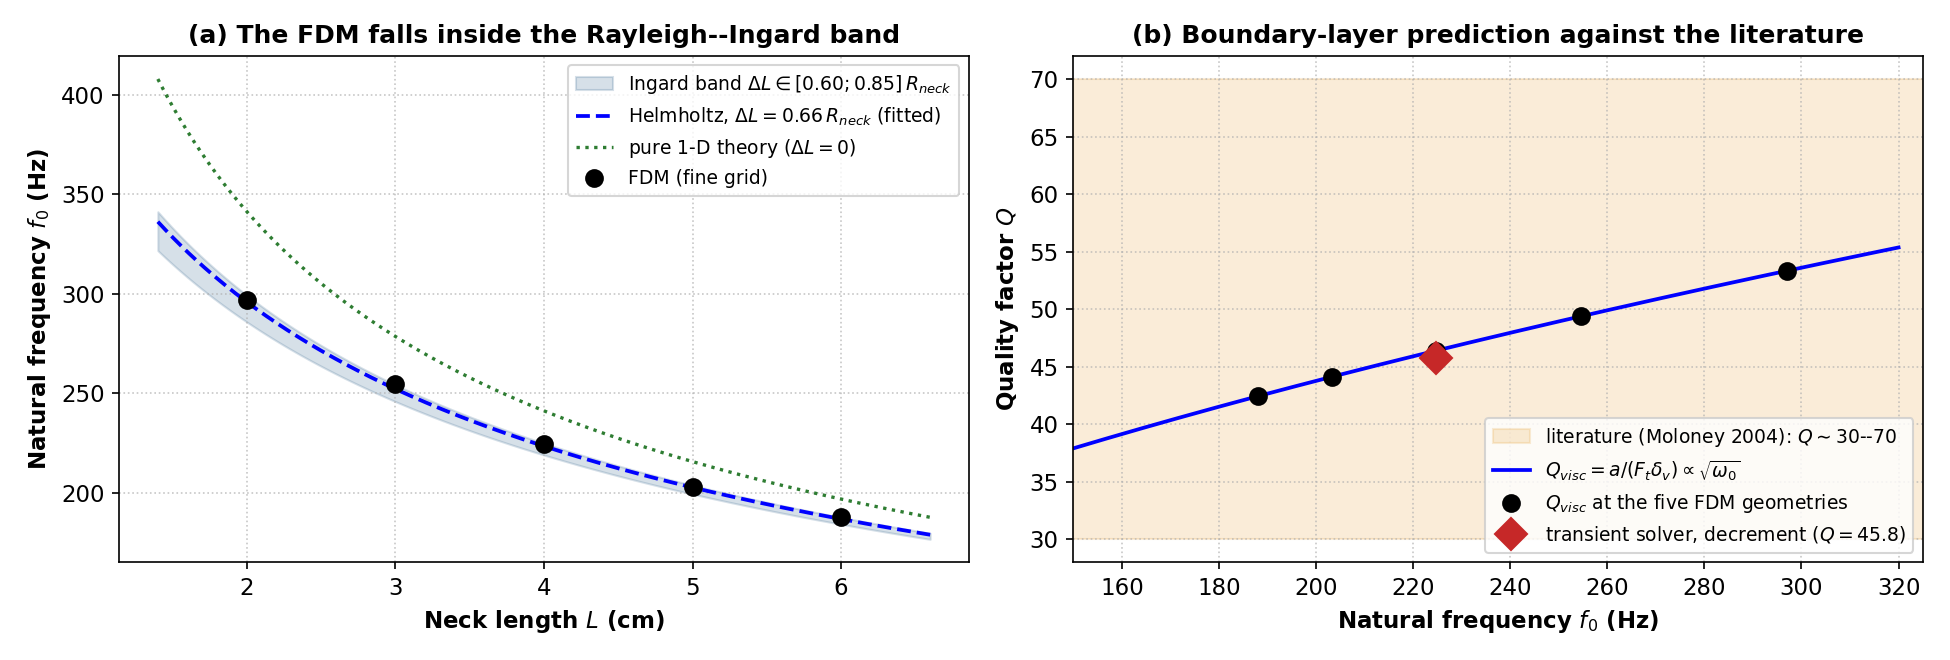
\includegraphics[width=0.92\textwidth]{phase2_verification.png}
\caption{Comparison with end corrections and quality factors from the literature. (a) The FDM frequencies fall inside the Rayleigh--Ingard band and far from the pure 1-D theory --- consistency, not independent verification. (b) The viscothermal quality factor $Q=R_{neck}/(F_t\delta_v)$ follows the $\sqrt{\omega_0}$ law; the transient-solver point ($Q=45.8$ by logarithmic decrement) and the range from the literature (Moloney 2004) are indicated.}
\label{fig:verif}
\end{figure*}

\section{Numerical Details and Reproducibility}
\label{sec:repro}
For reproducibility, the numerical parameters are as follows. The sparse linear system (CSR format, COO assembly) is solved by direct LU factorisation (\texttt{scipy.sparse.linalg.spsolve}, SuperLU) in complex double precision. The natural frequency is extracted by a coarse sweep ($2$ Hz step) followed by a fine sweep ($0.25$--$0.3$ Hz step over $\pm2.5$ Hz around the maximum) and a three-point parabolic interpolation; the stability of $f_0$ with respect to the sweep step is checked automatically (variation $<0.5$ Hz between steps of $1$ and $0.5$ Hz). The transient solver uses an explicit leapfrog scheme with $\Delta t = 0.85\,h/(c\sqrt{2})$ (that is $\mathrm{CFL}_{2D}=0.85$; $\Delta t \approx 3.5\ \mu$s at $h=2$ mm) over $60$ ms. The computations run on an x86-64 laptop (CPU only, single core) in Python/NumPy/SciPy. Every result and dataset of this article is regenerated by the self-contained notebook \texttt{etude\_helmholtz.ipynb}, which carries its own automatic checks (axis symmetry, resonance range, decrease of $f_0$ with $L$, stability with respect to the frequency step, MMS order); the figures are then redrawn from the stored data by \texttt{make\_paper\_figures.py}, so that the tables above and the plots below them come from one computation rather than two.

\section{Limitations and Conclusion}
The axisymmetric FDM solver developed here reproduces the expected decrease of the resonance frequency with neck length. The verification and validation are complete and hierarchical: the \emph{code} is verified by a manufactured solution (order $2.03$); the \emph{solution} by a GCI study on three grids, completed by a fourth control grid which confirms the stability of the observed order ($\approx 0.9$--$1.1$) and of the Richardson extrapolations ($0.01$--$0.32\%$ difference between triplets); the \emph{model} is given a first validation against two published experimental configurations ($0.9\%$ and $2.2\%$ deviation, with no fitted parameter). Once the numerical uncertainty ($\approx2\%$) is propagated into the weighted fit --- treated as a sensitivity analysis, the GCI not being a statistical standard deviation --- the power law and the effective-length model are \emph{indistinguishable} ($\Delta\text{AICc}$ not decisive, from $0.3$ to $1.8$ depending on the sample). The physical model is nevertheless preferred, because its constant ($A_H\approx A_H^{\mathrm{th}}$), its effective length ($\Delta L_{\mathrm{eff}} \approx 0.67$--$0.68\,R_{neck}$, of the same order as the Rayleigh--Ingard correction) and its out-of-sample prediction are all markedly better. These results are \emph{compatible} with the classical theory within the numerical uncertainty, without constituting a strict verification of it: $\Delta L_{\mathrm{eff}}$ remains an effective correction, and the apparent exponent $b \approx -0.42$ an artefact of a restricted geometric range. The radiation-impedance configuration (Section \ref{sec:radiation}) separates the interior part ($0.68\,R_{neck}$, the neck--cavity junction) from the exterior load, the measured shift ($0.823\,R_{neck}$) recovering the imposed baffled-piston reactance to $3.1\%$ --- a consistency test of the complete chain, to be distinguished from an \emph{ab initio} calculation of radiation. A reduced equivalent-damping model, calibrated on a viscothermal estimate ($Q\approx47$, compatible with the literature), illustrates the signatures of the losses without resolving them. A meshed exterior domain (Sommerfeld or PML \cite{berenger1994perfectly}) --- since carried out in the companion transient study --- a broader validation (several neck-to-cavity ratios, the full response) and a dedicated experimental campaign (protocol supplied with the repository) are the natural next steps.

\bibliographystyle{plain}
\bibliography{references}

\end{document}
